\documentclass[border=0.3cm, 12pt, convert = false]{standalone}
\usepackage{amsmath, amsthm, amssymb, amsfonts}
\usepackage{tikz}
\usepackage{helvet}
\renewcommand{\familydefault}{\sfdefault}

\begin{document}

  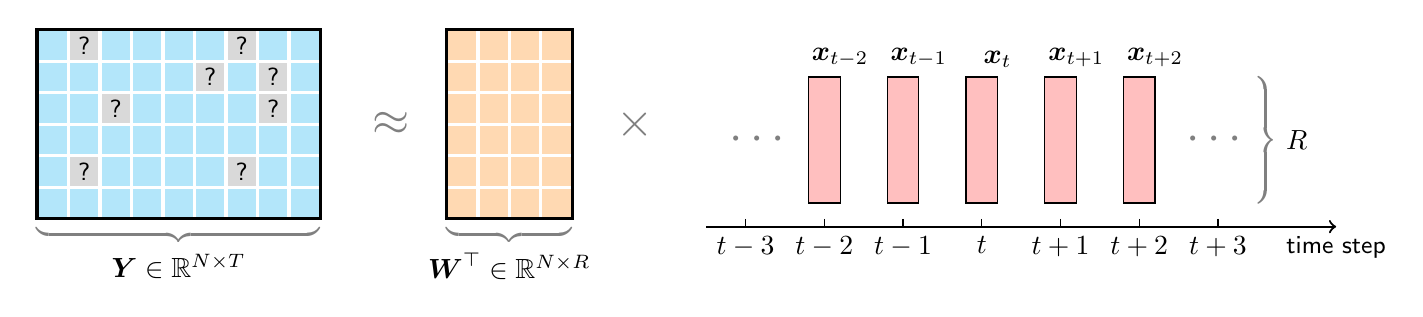
\begin{tikzpicture}[domain=0:4]
    \newcommand{\posx}{4}
    \newcommand{\posy}{3.8}

    \filldraw [fill=cyan!30!white,draw=green!40!black] (0,0-4) rectangle (3.6,2.4-4);
    \filldraw [fill=gray!30] (0.4,0.4-4) rectangle (0.8,0.8-4);
    \node at (0.6,0.6-4) {\small\color{black}?};
    \filldraw [fill=gray!30] (2.4,0.4-4) rectangle (2.8,0.8-4);
    \node at (2.6,0.6-4) {\small\color{black}?};
    \filldraw [fill=gray!30] (0.8,1.2-4) rectangle (1.2,1.6-4);
    \node at (1,1.4-4) {\small\color{black}?};
    \filldraw [fill=gray!30] (2.0,1.6-4) rectangle (2.4,2.0-4);
    \node at (2.2,1.8-4) {\small\color{black}?};
    \filldraw [fill=gray!30] (0.4,2.0-4) rectangle (0.8,2.4-4);
    \node at (0.6,2.2-4) {\small\color{black}?};
    \filldraw [fill=gray!30] (2.4,2.0-4) rectangle (2.8,2.4-4);
    \node at (2.6,2.2-4) {\small\color{black}?};
    \filldraw [fill=gray!30] (2.4,2.0-4) rectangle (2.8,2.4-4);
    \node at (2.6,2.2-4) {\small\color{black}?};
    \filldraw [fill=gray!30] (2.8,1.2-4) rectangle (3.2,2.0-4);
    \node at (3.0,1.4-4) {\small\color{black}?};
    \node at (3.0,1.8-4) {\small\color{black}?};
    \draw [step=0.4, very thick, color=white] (0,0-4) grid (4,2.4-4);
    \draw [very thick] (0,0-4) rectangle (3.6,2.4-4);
    \draw (1.8,-0.6-4) node {{\color{black}$\boldsymbol{Y}\in\mathbb{R}^{N\times T}$}};
    \draw (1.8,-0.2-4) node[rotate = 0] {{\color{gray}$\underbrace{\hspace{3.6cm}}$}};

    \draw (4.5,-2.8) node {\LARGE{\color{gray}$\approx$}};

    \filldraw [fill=orange!30!white,draw=black] (5.2,0-4) rectangle (6.8,2.4-4);
    \draw [step=0.4, very thick, color=white] (5.2,0-4) grid (6.8,2.4-4);
    \draw [very thick] (5.2,0-4) rectangle (6.8,2.4-4);
    \draw (6,-0.6-4) node {{\color{black}$\boldsymbol{W}^\top\in\mathbb{R}^{N\times R}$}};
    \draw (6,-0.2-4) node[rotate = 0] {{\color{gray}$\underbrace{\hspace{1.6cm}}$}};

    \draw (7.6,0.8-3.6) node[rotate = 0] {\LARGE\color{gray}$\times$};

    \draw (5+\posx,-0.2-\posy) -- (5+\posx,-0.3-\posy) node[anchor=north,fill=white] {$t-3$};
    \draw (6+\posx,-0.2-\posy) -- (6+\posx,-0.3-\posy) node[anchor=north,fill=white] {$t-2$};
    \draw (7+\posx,-0.2-\posy) -- (7+\posx,-0.3-\posy) node[anchor=north,fill=white] {$t-1$};
    \draw (8+\posx,-0.2-\posy) -- (8+\posx,-0.3-\posy) node[anchor=north,fill=white] {$t$};
    \draw (9+\posx,-0.2-\posy) -- (9+\posx,-0.3-\posy) node[anchor=north,fill=white] {$t+1$};
    \draw (10+\posx,-0.2-\posy) -- (10+\posx,-0.3-\posy) node[anchor=north,fill=white] {$t+2$};
    \draw (11+\posx,-0.2-\posy) -- (11+\posx,-0.3-\posy) node[anchor=north,fill=white] {$t+3$};
    \draw [->, thick] (4.5+\posx,-0.3-\posy) -- (12.5+\posx,-0.3-\posy) node [below] {\small time step};

    \draw (5.2+\posx,0.8-\posy) node[rotate = 0] {\LARGE\color{gray}$\cdots$};
    \filldraw [fill=red!25] (6-0.2+\posx,0-\posy) rectangle (6+0.2+\posx,1.6-\posy) node [above] {{\color{black}$\boldsymbol{x}_{t-2}$}};
    \filldraw [fill=red!25] (7-0.2+\posx,0-\posy) rectangle (7+0.2+\posx,1.6-\posy) node [above] {{\color{black}$\boldsymbol{x}_{t-1}$}};
    \filldraw [fill=red!25] (8-0.2+\posx,0-\posy) rectangle (8+0.2+\posx,1.6-\posy) node [above] {{\color{black}$\boldsymbol{x}_{t}$}};
    \filldraw [fill=red!25] (9-0.2+\posx,0-\posy) rectangle (9+0.2+\posx,1.6-\posy) node [above] {{\color{black}$\boldsymbol{x}_{t+1}$}};
    \filldraw [fill=red!25] (10-0.2+\posx,0-\posy) rectangle (10+0.2+\posx,1.6-\posy) node [above] {{\color{black}$\boldsymbol{x}_{t+2}$}};
    \draw (11+\posx,0.8-\posy) node[rotate = 0] {\LARGE\color{gray}$\cdots$};

    \draw (11.6+\posx,0.8-\posy) node[rotate = 90] {{\color{gray}$\underbrace{\hspace{1.6cm}}$}};
    \draw (12+\posx,0.8-\posy) node {{\color{black}$R$}};

\end{tikzpicture}

\end{document}
